\chapter{Umsetzung}
\label{ch:umsetzung}

\section{Datenbank}
\label{sec:datenbank}

\begin{figure}[htpb]
    \centering
    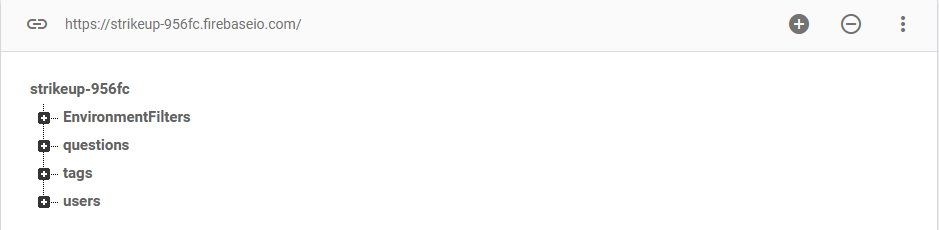
\includegraphics[width=0.85\textwidth]{db_minimiert}
    \caption{Minimierte Struktur der Datenbank}
    \label{img:db_minimiert}
\end{figure}
Daten werden in der Datenbank in Form vier verschiedener Kategorien gespeichert: \glqq{}EnvironmentFilters\grqq{} (Umgebungsvariablen), \glqq{}questions\grqq{} (Fragen),
\glqq{}tags\grqq{} (Tags) und \glqq{}users\grqq{} (Nutzer/-innen) (vgl. \ref{img:db_minimiert}).

Die Verwaltung der Datenbank erfolgt durch den Besitzer des Firebase-Projektes. Dies geschieht über eine Konsole. Um auf diese Konsole zuzugreifen, wird das entsprechende Google-Konto benötigt. \newline
Über die Konsole können in der Datenbank gespeicherte Daten beliebig geändert, gelöscht und hinzugefügt werden. Nutzerkonten können deaktiviert oder gelöscht werden. \newline
Bei einer Deaktivierung eines Nutezrkontos kann der/die entsprechende Nutzer/-in sich nicht mehr bei Strike Up anmelden. Des Weiteren kann eine Zurücksetzung des Passworts angefordert werden. \newline
Über die Konsole kann der aktuell genutzte Speicherplatz, sowie die in diesem und im vorherigen Monat heruntergeladene Datenmenge eingesehen werden. \newline
Zu den Nutzern/-innen werden (anonymisiert) das Land, in welchem sie Strike Up verwenden, das verwendete Betriebssystem, sowie die in der App verbrachte Zeit angezeigt. \newline
Außerdem können Zugriffsregeln für individuelle Abschnitte der Datenbank definiert werden.

Lese- und Schreibaufrufe werden im Code asynchron ausgeführt. Das bedeutet der Code \glqq{}läuft\grqq{} weiter, während der Lese-/Schreibaufruf im Hintergrund ausgeführt wird. Dies
verhindert das Finden von Fehlern mit einem \gls{debugger}, da Variablen, welche Daten aus der Datenbank enthalten, zur Laufzeit immer Null sind. Eine Fehlersuche im Zusammenhang mit
Leseaufrufen der Datenbank gestaltet sich somit schwierig. \newline
Wenn Daten aus der Datenbank in darauffolgendem Code benötigt werden, so muss auf die Fertigstellung des Lesevorgangs gewartet werden, da ansonsten mit Null-Objekten gearbeitet wird. Null-Objekte
würden zu Fehlern in der Anwendung führen. \newline
Ein Leseaufruf besteht aus einem \gls{listener}, welcher auf einen Knotenpunkt der Datenbank registriert wird. Beim Setzen eines \gls{listener}s (und wahlweise bei Veränderung der Daten
unter dem registrierten Knotenpunkt) wird dessen Funktion einmal ausgeführt. Um Null-Objekte zu verhindern, werden, auf einen Leseaufruf folgende, Funktionen in dem zugehörigen \gls{listener}
aufgerufen. Dies umgeht das asynchrone Ausführen der Leseaufrufe. Bei mehrern aufeinanderfolgenden Leseaufrufen, verzögert sich jedoch die Ausführung des Codes, da bei jedem Aufruf auf
dessen Fertigstellung gewartet wird. Dies kann in Extremfällen, und bei langsamem Internet, die Ausführung der App verlangsamen.


\section{Nutzerprofile}
\label{sec:profile}

Damit Nutzer/-innen Zugriff auf die von Strike Up bereitgestellten Funktionen haben, müssen sie sich zuerst registrieren. Eine Registrierung verhindert, in beschränktem Maße, dass die
von Strike Up genutzte Datenbank mit ungenutzten Nutzerprofilen gefüllt wird. Dies spart Speicherplatz, welcher im kostenlosen Vertrag beschränkt ist.
\begin{figure}[htpb]
    \centering
    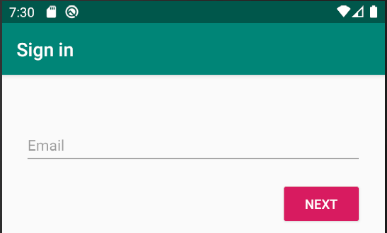
\includegraphics[width=0.5\textwidth]{Sign_in}
    \caption{Anmeldung mit E-Mail-Adresse}
    \label{img:signin_email}
\end{figure}
\begin{figure}[htpb]
    \centering
    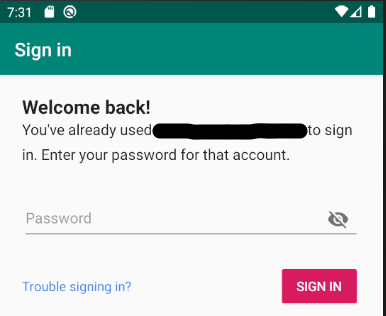
\includegraphics[width=0.5\textwidth]{sign_in_password}
    \caption{Aufforderung zur Eingabe des Passworts}
    \label{img:signin_password}
\end{figure}
Die Anmeldung erfolgt über eine E-Mail-Adresse und ein Passwort (siehe \ref{img:signin_email} und \ref{img:signin_password}). Ist die E-Mail-Adresse bereits auf ein Konto registriert, so
wird der/die Nutzer/-in aufgefordert das dazugehörige Passwort einzugeben (\ref{img:signin_password}). Wenn mit der E-Mail-Adresse ein neues Konto angelegt wird, so muss der/die Nutzer/-in
ein neues Passwort für diesen Account festlegen.

In der Datenbank werden Nutzer/-innen unter ihrer \gls{uid} gespeichert. Die \gls{uid} ist eine einzigartige, von Firebase automatisch generierte Kennung. Anhand dieser einzigartigen
Kennung wird jede/-r Nutzer/-in von Strike Up identifiziert. Wird eine Nutzeraccount gelöscht, so wird auch dessen \gls{uid} entfernt.

Abgesehen von der \gls{uid} besitzt ein Nutzerprofil folgende Attribute:
\begin{itemize}
    \item Name: Der Name des/der Nutzers/-in
    \item Email: Die E-Mail-Adresse des/der Nutzers/-in
    \item Alter: Das Alter des/der Nutzers/-in
    \item PreferredTags: Eine Liste aller Tags, welche der/die Nutzer/-in bevorzugt
    \item IgnoredTags: Eine Liste aller Tags, welche der/die Nutzer/-in vermeiden will
    \item ConversationalPartners: Eine Liste aller gespeicherten Gesprächspartner/-innen (siehe \ref{subsec:gespraechspartner}) des/der Nutzers/-in
\end{itemize}


\subsection{Tags}
\label{subsec:tags}

Tags werden in der Datenbank unter dem Knoten \glqq{}tags\grqq{} gespeichert. Ein Tag besitzt keine Attribute. Tags sind für jeden authentifizierten Nutzer einsehbar.

Nutzer/-innen wählen aus der Liste aller verfügbaren Tags aus, ob ihnen ein Tag gefällt oder nicht. Das Auswählen der bevorzugten und gemiedenen Tags geschieht dabei über zwei separate
Buttons. \newline
Tags, welche bereits in der Liste bevorzugter Tags sind, werden beim Hinzufügen neuer bevorzugter Tags nicht mehr zur Auswahl angeboten. Das Gleiche gilt für gemiedene Tags. Beim Hinzufügen
neuer bevorzutger Tags werden jedoch auch Tags angezeigt, welche in der Liste gemiedener Tags vorhanden sind. Dies gilt auch umgekehrt. \newline
\begin{figure}[htpb]
    \centering
    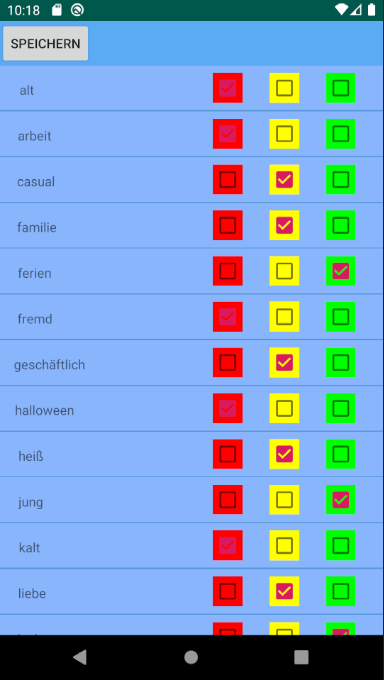
\includegraphics[width=0.35\textwidth]{alle_tags}
    \caption{Auswahl bevorzugter und gemiedener Tags}
    \label{img:alle_tags}
\end{figure}
Damit Tags nur in einer Liste vorkommen, und um die Auswahl der Tags zu vereinfachen, wird eine neue Funktion entwickelt, welche über mehrere Checkboxen das Aufteilen der Tags in die
entsprechenden Listen ermöglicht (\ref{img:alle_tags}). Rot steht dabei für gemiedene Tags und grün für bevorzugte Tags. Gelb markierte Tags sind in keiner der beiden Listen vorhanden und werden somit neutral bewertet. \newline
Ein Problem tut sich dabei bei der Implementation einer \gls{listactivity} in Android auf. Da mehr Objekte in der anzuzeigenden Liste sind, als auf den Bildschirm passen, verwendet Android
bereits für angezeigte Elemente verwendete \gls{container}, um noch nicht angezeigte Elemente zu laden \cite{misc:android_listview}. Das bedeutet: Wenn ein, mit einem Objekt gefüllter,
\gls{container} (durch scrollen) vom Bildschirm verschwindet, wird dieser \gls{container} benutz um das neu erschienene Element anzuzeigen. Der \gls{container} behält dabei die
Position des Hakens der Checkbox. Beim Scrollen, wird somit bei neu erschienen Tags der Haken an der Position der neu ausgeblendeten Tags gesetzt. Dies lässt sich durch das Verwenden
einer \gls{hashmap}, welche die Positionen der Haken speichert, umgehen. Dabei ist der Name eines Tags der \glqq{}Key\grqq{} und die Position des Hakens das \glqq{}Value\grqq{}. \newline
Aus Zeitgründen ist diese Funktion noch nicht fehlerfrei lauffähig. Deshalb geschieht die Auswahl bevorzugter und gemiedener Tags weiterhin über zwei separate Buttons.

Während der Entwicklung wurden Tags um eine ID erweitert; Tags werden somit unter ihrer ID gespeichert und besitzen das Attribut \glqq{}Name\grqq{}. \newline
Das Verwenden einer ID ermöglicht, dass Strike Up auf weitere Sprachen erweitert werden kann. So können Tags beispielsweise um die Attribute \glqq{}Name-en\grqq{} oder \glqq{}Name-fr\grqq{} erweitert
werden.

\subsection{Gesprächspartner/-innen}
\label{subsec:gespraechspartner}

Gesprächspartner/-innen werden als eine, zu einem/-r Nutzer/-in gehörende, Liste gespeichert. Jede/-r Nutzer/-in kann beliebig viele Gesprächspartner/-innen hinzufügen. \newline
Ein/-e Gesprächspartner/-in besitzt die Attribute:
\begin{itemize}
    \item Name: Name des/der Gesprächspartners/-in
    \item Gender: Geschlecht des/der Gesprächspartners/-in
    \item Alter: Alter des/der Gesprächspartners/-in
    \item IgnoredTags: Eine Liste aller Tags, welche der/die Gesprächspartner/-in vermeiden will
    \item PreferredTags: Eine Liste aller Tags, welche der/die Gesprächspartner/-in bevorzugt
    \item Notizen: Von dem/der Nutzer/-in verfasste Notizen zu dem/der Gesprächspartner/-in
\end{itemize}
Das Bearbeiten und Auswählen von Tags geschieht dabei gleich wie bei einem/-r Nutzer/-in.

Gesprächspartner/-innen werden um das Atttribut ID erweitert, da sie bisher unter ihrem Namen in der Datenbank gespeichert wurden. Das Speichern unter dem Namen erzeugte Probleme, wenn
der Name geändert wurde, da so zwei Objekte desselben Partnerprofils in der Datenbank hinterlegt waren. Gebraucht wird aber nur ein Objekt. Es entsanden also redundante Daten. \newline
Das Einführen einer unveränderlichen und einzigartigen ID ermöglicht eine problemfreie Änderung des Namens. \newline
Die ID wird von Firebase generiert. Zum erstellen dieser einzigartigen ID benutzt Firebase den gewünschten Speicherort innerhalb der Datenbank und das aktuelle Datum.

Nachdem das Profil eines/-r Gesprächspartners/-in erstellt ist, kann dieses bearbeitet und wieder gelöscht werden.

Strike Up besitzt individuelle Profile für den/die Nutzer/-in und für Gesprächspartner/-innen. Somit ist F-6 erfüllt (vgl. \ref{tab:funktional}).


\section{Fragen/Hinweise}
\label{sec:fragen_hinweise}

Fragen und Hinweise werden in der Datenbank unter \glqq{}questions\grqq{} gespeichert. Eine einzelne Frage ist dabei unter ihrer ID zu finden. \newline
Fragen besitzen folgende Attribute:
\begin{itemize}
    \item ID: Eine eindutige ID, unter welcher die Frage gespeichert ist
    \item tags: Eine Liste aller Tags, welche zu dieser Frage passen
    \item text: Der Text der Frage
\end{itemize}
Fragen und Hinweise können nicht von Nutzern/-innen bearbeitet werden. Das Verändern, Hinzufügen und Entfernen von Fragen obliegt somit dem/der Verwalter/-in der Datenbank. \newline
Ursprünglich war geplant, dass Nutzer/-innen sowohl Fragen als auch Tags zur Datenbank hinzufügen können, da die Datenbank besonders in den Anfängen von Strike Up noch nicht vollständig
ist. Diese Idee wurde jedoch aus Angst vor Missbrauch wieder gestrichen.

\subsection{Umgebungsvariablen}
\label{subsec:umgebungsvariablen}

Eine Umgebungsvariable wird mit folgenden Attributen in der Datenbank gespeichert:
\begin{itemize}
    \item ID: Eine eindutige ID, unter welcher die Umgebungsvariable gespeichert ist
    \item Name: Der Name der Umgebungsvariable
    \item IgnoredTags: Liste aller Tags, auf welche die Umgebungsvariable einen negativen Einfluss hat
    \item Preferred Tags: Liste aller Tags, auf welche die Umgebungsvariable einen positiven Einfluss hat
\end{itemize}
Umgebungsvariablen werden vor einem Gepräch entweder automatisch generiert oder durch den/die Nutzer/-in gesetzt. \newline
Die Umgebungsvariable Alter (jung/alt) wird automatisch generiert und der/die Nutzer/-in kann die Umgebungsvariable \glqq{}Privat\grqq{} oder \glqq{}Geschäftlich\grqq{}
auswählen. Alternativ kann die Auswahl einer Umgebungsvariable auch übersprungen werden. \newline
Das automatische Generieren und manuelle Auswählen von Umgebungsvariablen ist noch erweiterbar. Die bisherige Implementation stellt einen konzeptionellen Beweiß der Erfüllbarkeit von F-13 dar.

Im Laufe der Arbeit kam auf, dass die Eingabe eines statischen Alters bei Nutzerprofilen und Gesprächspartnern/-innen nicht sinnvoll ist, da sich dieses jährlich ändert.
Fragen und Hinweise beziehen sich auf das Alter und Strike Up setzt automatisch Umgebungsvariablen zu diesem (z.B. Jung oder Alt). Aus diesem Grund wird Alter als Profil-Attribut entfernt.
Stattdessen wird das Geburtsdatum verwendet. Aus diesem wird, bei einem Datenbankabruf des Profils, das Alter ermittelt. Somit aktualisiert sich das Alter eines Profils am Geburtstag.


\section{Gespräch}
\label{sec:gespräch}

Vor einem Gespräch wird aus der Liste aller verfügbaren Gesprächspartner/-innen ein/-e Gesprächspartner/-in ausgewählt oder alternativ ein/-e neue/-r Gesprächspartner/-in erstellt.
Anschließend kann der/die Gesprächspartner/-in noch einmal bearbeitet werden. Bevor die Konversation beginnt wählt der/die Nutzer/-in noch manuell Umgebungsvariablen aus.

Die Listen bevorzugter Tags des/der Nutzers/-in, des Gegenübers und der Umgebungsvariablen werden addiert. Doppelte (dreifache, vierfache, \dots) Tags sind dabei erlaubt. Das Gleiche passiert
mit den entsprechenden Listen gemiedener Tags. \newline
Ist die Listen fertig, so wird diese mit den entsprechenden Listen jeder verfügbaren Frage verglichen. Hierfür werden alle Tags der bevorzugten/gemiedenen Listen einzeln
miteinander verglichen. \newline
Kommt ein Tag sowohl in der Liste der bevorzugten (gemiedenen) Tags einer Frage, als auch in der kombinierten Liste bevorzugter Tags von Nutzers/-in, Gegenüber und Umgebungsvariablen vor,
so wird bei der Frage ein Punkt addiert (subtrahiert). Fragen starten dabei mit einer Punktzahl von null.

\begin{figure}[htpb]
    \centering
    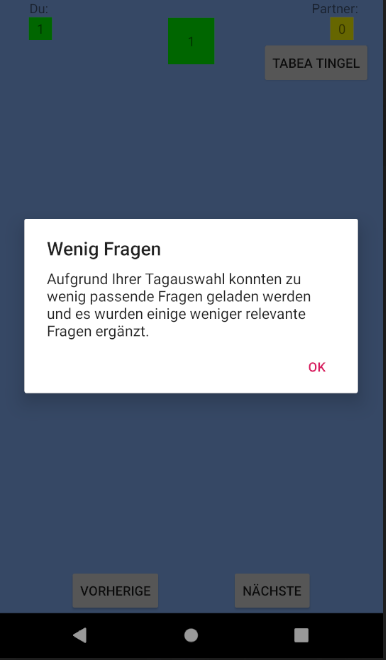
\includegraphics[width=0.35\textwidth]{warning_conversation}
    \caption{Warnung, wenn weniger relevante Fragen hinzugefügt werden}
    \label{img:warning_conversation}
\end{figure}

Für die Konversation werden nur Fragen mit einer Punktzahl über null ausgewählt. Sollten somit jedoch weniger als zehn Fragen verfügbar sein, so werden auch Fragen mit einer Punktzahl von null
hinzugefügt. Sind immer noch weniger als zehn Fragen vorhanden, so werden auch negativ bewertete Fragen hinzugefügt. Der/die Nutzer/-in wird durch ein \gls{popup} auf diesen Umstand aufmerksam gemacht
(vgl. \ref{img:warning_conversation}).

Während einem Gespräch sieht die \gls{ui} wie in \ref{img:conversation} aus. Über die Buttons \glqq{}vorherige\grqq{} und \glqq{}nächste\grqq{} kann zwischen den für das Gespräch
verfügbaren Fragen gewechselt werden (F-5). Der Text der Fragen wird zentral im Bildschirm angezeigt, während andere Funktionen, wie Buttons, am Rand vorhanden sind (NF-3).
\begin{figure}[htpb]
    \centering
    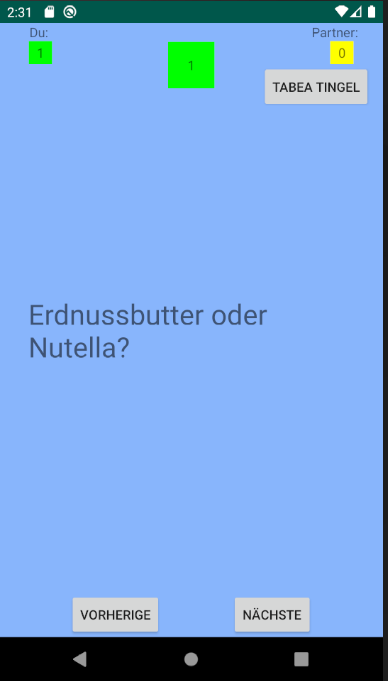
\includegraphics[width=0.35\textwidth]{conversation}
    \caption{Frage während einer Konversation}
    \label{img:conversation}
\end{figure}
Das farbige Quadrat unter \glqq{}Du\grqq{} zeigt die Bewertung der Frage aus Sicht des Nutzers an. Das Quadrat unter \glqq{}Partner\grqq{} zeigt die Bewertung aus Sicht des Gegenübers
und das große Quadrat zeigt die Gesamtbewertung. Eine grüne Farbe steht dabei für eine positive, gelb für eine neutrale und rot für eine negative Bewertung.

Über \glqq{}Tabea Tingel\grqq{} wird das Profil des Gegenübers aufgerufen. Somit sind Notizen des Gegenübers während einem Gespräch verfügbar (F-7). Das Profil des/der Gesprächspartners/-in
kann somit auch erst während einer Konversation mit Informationen befüllt werden.


\section{Datenschutz}
\label{sec:datenschutz}

Strike Up soll keine personenbezogenen Daten an Dritte weitergeben (vgl. \ref{tab:nichtfunktional}, NF-4). Als \glqq{}Dritte\grqq{} ist hierbei Google in der Rolle des Verwalter der Daten,
zu verstehen. \newline
Google ist hierbei ein \glqq{}processor of [...] Customer Personal Data under the European Data Protection Legislation\grqq{} \cite{misc:firebase_terms}. Dies bedeutet, dass Google ein
Verwalter der Daten ist, diese aber nicht einsehen oder versenden darf. \newline
Da die zu Strike Up gehörende Datenbank von der EU aus bearbeitet wird, gilt die \gls{dsgvo}. Somit muss Google Daten an Behörden weiterleiten, falls dies gefordert wird.

Des Weiteren ist der Ersteller von Strike Up für das Einhalten der \gls{dsgvo} verantwortlich. Um dies zu garantieren wird beim ersten Öffnen der Anwendung ein Dialogfenster geöffnet,
welches den/die nutzer/-in auffordert zu bestätigen, dass er/sie über 18 Jahre alt ist. Außerdem willigt er/sie ein, dass alle von Strike Up verarbeiteten Daten gespeichert werden. \newline
Wird eine dieser zwei Bedienungen nicht erfüllt, so schließt sich Strike Up und der Ablauf wird beim nächsten Öffnen wiederholt.

\subsection{Schutz vor Datendiebstahl}
\label{subsec:datendiebstahl}

Damit Strike Up auf die Cloud-Datenbank zugreifen kann, wird eine \gls{url} zu dieser benötigt. Die \gls{url} ist dabei im Code der Anwendung enthalten. \newline
Diese \gls{url} ermöglicht Angreifern jedoch keinen Zugriff auf die Datenbank, da zudem noch das verbundene Google-Konto benötigt wird.

Eine weitere Angriffsmöglichkeit ist der im Quellcode hinterlegte \gls{api}-Key, welcher Strike Up bei der Datenbank registriert. Über den \gls{api}-Key können Angreifer auf alle in der
Datenbank gespeicherten Daten zugreifen. \newline
Dies wird durch das Aufstellen von Regeln verhindert. Regeln beziehen sich auf definierte Bereiche der Datenbank. Die für Strike Up definierten Regeln erlauben
jedem/-r authentifizierten Nutzer/-in das Lesen der Bereiche \glqq{}EnvironmentFilters\grqq{}, \glqq{}questions\grqq{} und \glqq{}tags\grqq{} (vgl. \ref{img:db_minimiert}). \newline
Da der Bereich \glqq{}users\grqq{} nutzerspezifische Daten enthält, ist nicht jedem/-r Nutzer/-in erlaubt alle darunter liegenden Knoten zu lesen. Jede/-r Nutzer/-in kann dabei nur auf
\glqq{}unter\grqq{} seiner/ihrer \gls{uid} gespeicherte Daten zugreifen. Der/die Nutzer/-in hat für diesen Bereich Lese- und Schreibrechte.